\section{CLIP: Kết nối Ảnh và Ngôn ngữ}
\label{sec:clip}

Trước năm 2021, các mô hình thị giác máy tính hàng đầu, dù mạnh mẽ đến đâu, vẫn hoạt động trong một "thế giới câm". Chúng có thể phân loại một bức ảnh về một con chó với độ chính xác cao, nhưng chúng không "biết" rằng các pixel đó tương ứng với khái niệm được biểu thị bằng chuỗi ký tự "c-h-ó". Sự kết nối giữa thế giới thị giác phong phú và thế giới ngôn ngữ trừu tượng vẫn còn rất lỏng lẻo.

\textbf{CLIP (Contrastive Language-Image Pre-training)} \cite{Radford2021}, một công trình đột phá từ OpenAI, đã thay đổi hoàn toàn điều đó. Nó là một trong những mô hình nền tảng đa phương thức (multimodal foundation model) quy mô lớn đầu tiên, đã tạo ra một cầu nối vững chắc và có ý nghĩa giữa hình ảnh và văn bản.

\subsection{Ý tưởng Cốt lõi: Học từ Web}
\label{subsec:clip_core_idea}
Thay vì học từ các bộ dữ liệu được gán nhãn thủ công với các lớp cố định (như ImageNet), CLIP được huấn luyện trên một nhiệm vụ đơn giản hơn nhưng ở quy mô lớn hơn rất nhiều: \textbf{dự đoán xem một chú thích văn bản (caption) có tương ứng với một hình ảnh cho trước hay không}.

\textbf{Dữ liệu:} Các nhà nghiên cứu đã thu thập một bộ dữ liệu khổng lồ gồm \textbf{400 triệu cặp (ảnh, văn bản)} từ internet. Các cặp này không được làm sạch hay gán nhãn một cách cẩn thận; chúng chỉ đơn giản là các hình ảnh và các đoạn văn bản "alt-text" đi kèm với chúng. Sự đa dạng và hỗn loạn của dữ liệu web này chính là chìa khóa cho khả năng khái quát hóa mạnh mẽ của CLIP.

\subsection{Kiến trúc và Phương pháp Huấn luyện Tương phản}
\label{subsec:clip_architecture_training}
CLIP bao gồm hai thành phần chính:
\begin{enumerate}
	\item \textbf{Image Encoder:} Một mạng nơ-ron (có thể là một ResNet hoặc một Vision Transformer - ViT) nhận đầu vào là một bức ảnh và tạo ra một vector nhúng (embedding vector) cho ảnh đó, ký hiệu là $\mathbf{I}_e$.
	\item \textbf{Text Encoder:} Một kiến trúc Transformer tiêu chuẩn nhận đầu vào là một chuỗi văn bản (đã được token hóa) và tạo ra một vector nhúng cho văn bản, ký hiệu là $\mathbf{T}_e$.
\end{enumerate}

\textbf{Huấn luyện Tương phản (Contrastive Learning):}
Mục tiêu của quá trình huấn luyện là học một \textbf{không gian nhúng đa phương thức (multimodal embedding space)} chung, nơi các biểu diễn của ảnh và văn bản tương ứng có thể được so sánh trực tiếp.
\begin{itemize}
	\item Trong một mini-batch gồm $N$ cặp (ảnh, văn bản), chúng ta sẽ có $N$ embedding ảnh $\{\mathbf{I}_1, ..., \mathbf{I}_N\}$ và $N$ embedding văn bản $\{\mathbf{T}_1, ..., \mathbf{T}_N\}$.
	\item Độ tương đồng giữa một ảnh $i$ và một văn bản $j$ được tính bằng \textbf{độ tương đồng cosine (cosine similarity)}.
	\item \textbf{Mục tiêu:} Mô hình được huấn luyện để tối đa hóa độ tương đồng của $N$ cặp (ảnh, văn bản) tương ứng trên đường chéo chính (ví dụ: $(\mathbf{I}_i, \mathbf{T}_i)$) và đồng thời tối thiểu hóa độ tương đồng của $N^2 - N$ cặp không tương ứng còn lại (ví dụ: $(\mathbf{I}_i, \mathbf{T}_j)$ với $i \neq j$).
	\item \textbf{Hàm mất mát:} Quá trình này được tối ưu hóa bằng một hàm mất mát tương phản đối xứng (symmetric contrastive loss), về cơ bản là tính trung bình của hai hàm mất mát cross-entropy: một cho dự đoán văn bản từ ảnh, và một cho dự đoán ảnh từ văn bản.
\end{itemize}

\begin{center}
	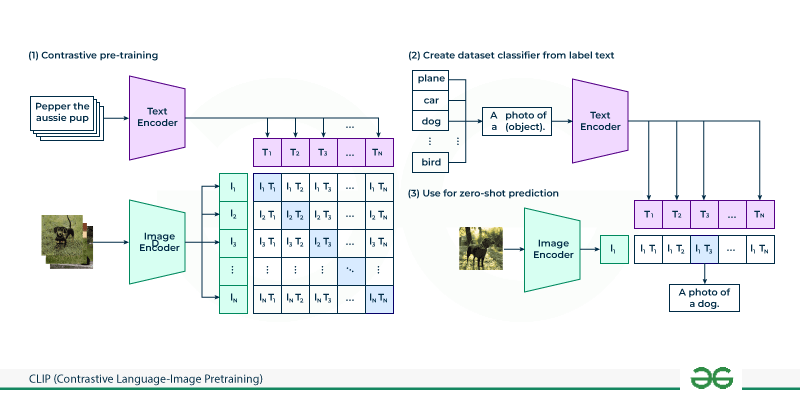
\includegraphics[width=1.0\textwidth]{images/clip_contrastive_pretraining.png}
	\captionof{figure}{Sơ đồ quá trình huấn luyện tương phản của CLIP. Trong một batch, mô hình cố gắng khớp đúng các cặp (ảnh, văn bản) tương ứng (trên đường chéo) và phân biệt chúng với tất cả các cặp không tương ứng khác.}
	\label{fig:clip_pretraining}
\end{center}
% Keyword gợi ý: clip contrastive pretraining, clip architecture diagram

\subsection{Phép màu của Zero-Shot Classification}
\label{subsec:clip_zero_shot}
Sức mạnh thực sự của CLIP không nằm ở kiến trúc, mà ở khả năng thực hiện các tác vụ một cách \textbf{zero-shot}—tức là không cần bất kỳ sự tinh chỉnh (fine-tuning) nào trên bộ dữ liệu của tác vụ đó.

\textbf{Quy trình Phân loại Ảnh Zero-Shot:}
Để phân loại một bức ảnh vào một trong $M$ lớp, CLIP thực hiện một quy trình đơn giản và thanh lịch:
\begin{enumerate}
	\item \textbf{Chuẩn bị Prompt Văn bản:} Tạo một tập hợp các prompt văn bản mô tả từng lớp. Ví dụ, đối với các lớp "dog", "cat", "car", chúng ta tạo các câu như: \texttt{"a photo of a dog"}, \texttt{"a photo of a cat"}, \texttt{"a photo of a car"}. Việc sử dụng các câu hoàn chỉnh thay vì chỉ các từ đơn lẻ giúp mô hình hiểu ngữ cảnh tốt hơn.
	\item \textbf{Mã hóa:}
	\begin{itemize}
		\item Đưa ảnh cần phân loại qua Image Encoder để thu được vector $\mathbf{I}_e$.
		\item Đưa tất cả $M$ prompt văn bản qua Text Encoder để thu được $M$ vector $\{\mathbf{T}_{e,1}, ..., \mathbf{T}_{e,M}\}$.
	\end{itemize}
	\item \textbf{So khớp và Dự đoán:}
	\begin{itemize}
		\item Tính toán độ tương đồng cosine giữa $\mathbf{I}_e$ và mỗi vector $\mathbf{T}_{e,j}$.
		\item Áp dụng một hàm softmax trên các điểm số tương đồng này để tạo ra một phân phối xác suất.
		\begin{equation}
			p(y=j|\mathbf{x}) = \frac{\exp(\text{sim}(\mathbf{I}_e, \mathbf{T}_{e,j}) / \tau)}{\sum_{k=1}^{M} \exp(\text{sim}(\mathbf{I}_e, \mathbf{T}_{e,k}) / \tau)}
		\end{equation}
		\item Lớp có xác suất cao nhất được chọn làm dự đoán cuối cùng.
	\end{itemize}
\end{enumerate}
Khả năng này đã làm thay đổi hoàn toàn cách tiếp cận các bài toán phân loại. Thay vì phải huấn luyện một mô hình chuyên biệt cho từng bộ dữ liệu, người ta có thể sử dụng CLIP "ngay lập tức" trên hàng chục bộ dữ liệu khác nhau và vẫn đạt được hiệu năng rất cạnh tranh.

\subsection{Ứng dụng và Tầm ảnh hưởng}
\label{subsec:clip_applications_impact}
CLIP không chỉ là một bộ phân loại zero-shot mạnh mẽ. Các biểu diễn đa phương thức mà nó học được đã trở thành một thành phần nền tảng, một "xương sống" cho vô số các mô hình và ứng dụng tiên tiến khác:

\begin{itemize}
	\item \textbf{Tìm kiếm Ảnh bằng Văn bản (Text-to-Image Retrieval):} Đây là ứng dụng tự nhiên nhất. Bằng cách mã hóa một câu truy vấn và tìm kiếm các embedding ảnh gần nhất, CLIP đã tạo ra các hệ thống tìm kiếm hình ảnh dựa trên ngữ nghĩa cực kỳ mạnh mẽ.
	\item \textbf{Nền tảng cho các Mô hình Sinh:} Các mô hình tạo ảnh từ văn bản như DALL-E 2, Stable Diffusion, và Midjourney sử dụng các text encoder của CLIP (hoặc các biến thể của nó) để "hiểu" prompt của người dùng và hướng dẫn quá trình sinh ảnh.
	\item \textbf{Xương sống cho các Tác vụ Thị giác Phức tạp:} Các đặc trưng từ Image Encoder của CLIP đã được chứng minh là cực kỳ hiệu quả khi được sử dụng làm backbone cho các tác vụ như phát hiện vật thể (ví dụ: \textbf{Grounding DINO}), phân đoạn ảnh (ví dụ: \textbf{CLIPSeg}), và các Mô hình Ngôn ngữ Lớn Đa phương thức (LVLMs).
\end{itemize}

\subsection{Hạn chế và Tương lai}
\label{subsec:clip_limitations_future}
Mặc dù mang tính cách mạng, CLIP vẫn có những hạn chế:
\begin{itemize}
	\item \textbf{Thiên vị từ Dữ liệu Web:} Do được huấn luyện trên dữ liệu internet không được lọc kỹ, CLIP có thể học và khuếch đại các thiên vị xã hội (social biases) có trong dữ liệu đó.
	\item \textbf{Hiểu biết Chi tiết Hạn chế:} CLIP xuất sắc trong việc nhận dạng các đối tượng chính, nhưng thường gặp khó khăn với các tác vụ đòi hỏi sự hiểu biết chi tiết, như đếm số lượng đối tượng, đọc văn bản trong ảnh, hoặc lý luận về các mối quan hệ không gian phức tạp.
	\item \textbf{Nhạy cảm với Prompt (Prompt Sensitivity):} Hiệu năng zero-shot của CLIP có thể thay đổi đáng kể tùy thuộc vào cách một prompt được viết. Lĩnh vực "prompt engineering" đã ra đời một phần để giải quyết vấn đề này.
\end{itemize}
Dù vậy, CLIP đã mở ra một kỷ nguyên mới. Nó chứng minh rằng bằng cách học trên quy mô lớn từ sự kết hợp tự nhiên giữa hình ảnh và ngôn ngữ, chúng ta có thể xây dựng các mô hình thị giác có khả năng khái quát hóa và linh hoạt chưa từng có. Nó đã đặt nền móng vững chắc cho sự hội tụ của thị giác và ngôn ngữ, một xu hướng đang định hình nên tương lai của trí tuệ nhân tạo.

\section*{Tài liệu tham khảo}
\begin{itemize}
	\item[1] Radford, A., Kim, J. W., Hallacy, C., Ramesh, A., Goh, G., Agarwal, S., ... \& Sutskever, I. (2021). Learning transferable visual models from natural language supervision. In \textit{International Conference on Machine Learning (ICML)}. (Paper gốc và kinh điển giới thiệu CLIP).
	\item[2] Ilharco, G., Wortsman, M., Wightman, R., Gordon, C., Carlini, N., ... \& Schmidt, L. (2021). Openclip. \textit{https://github.com/mlfoundations/open\_clip}. (Dự án mã nguồn mở tái tạo và mở rộng CLIP, một nguồn tài nguyên quan trọng cho cộng đồng).
	\item[3] Jia, C., Yang, Y., Xia, Y., Chen, Y. T., Parekh, Z., Pham, H., ... \& Duerig, T. (2021). Scaling up visual and vision-language representation learning with noisy text supervision. In \textit{International Conference on Machine Learning (ICML)}. (Paper giới thiệu ALIGN, một mô hình tương tự CLIP từ Google, được huấn luyện trên quy mô lớn hơn).
	\item[4] Dosovitskiy, A., Beyer, L., Kolesnikov, A., Weissenborn, D., Zhai, X., Unterthiner, T., ... \& Houlsby, N. (2020). An image is worth 16x16 words: Transformers for image recognition at scale. \textit{arXiv preprint arXiv:2010.11929}. (Paper về Vision Transformer, kiến trúc image encoder được sử dụng trong các phiên bản CLIP mạnh nhất).
\end{itemize}